\frontmatter												%Seitennumerierung
\pagenumbering{Roman}										%Römische Zahlen
\addtocounter{page}{2}

\newcommand{\doublesignature}[2]{%
  \parbox{\textwidth}{
    \hfill
    \parbox{7cm}{
      \centering
      \rule{6cm}{1pt}\\
      #1
    }
    \parbox{7cm}{
      \centering
      \rule{6cm}{1pt}\\
      #2
    }
  }
  \mbox{}\\
  \mbox{}\\
  \mbox{}\\
  \mbox{}\\
}

\vspace*{20pt}

\section*{Eidesstattliche Erklärung}
\label{sec:eidesstattliche-erklaerung}
Ich erkläre an Eides statt, dass ich die vorliegende Arbeit selbstständig verfasst, andere als die angegebenen
Quellen/Hilfsmittel nicht benutzt und die den benutzten Quellen wörtlich und inhaltlich entnommenen
Stellen als solche kenntlich gemacht habe.\\
\\
Arnfels, am 5. April 2018\\

\vskip 1cm

\doublesignature{Stefan Hörmann}{Nicolas Perl}
\doublesignature{Alois Vollmaier}{Mr. Mösensaft}

\vskip 5cm

\clearpage

\newpage
\thispagestyle{empty}
\mbox{}

\clearpage

\section*{Danksagung}
\label{sec:danksagung}
An dieser Stelle möchten wir uns bei allen bedanken, die uns im Rahmen der Diplomarbeit unterstützt und betreut haben.\\
\\
TODO

\clearpage

\newpage
\thispagestyle{empty}
\mbox{}

\clearpage

\section*{Abstract}
\label{sec:abstract}
TODO

\section*{Zusammenfassung}
Wir setzten uns als Ziel eine Maschine zu entwickeln, welche das Mischen, sowie das Ausgeben von Spielkarten übernimmt.
Die Idee ist es, diese Verfahren möglichst platzsparend, zeiteffizient und detailliert durchdacht und optimiert zu realisieren.\\


\begin{figure}[H]
  \centering
  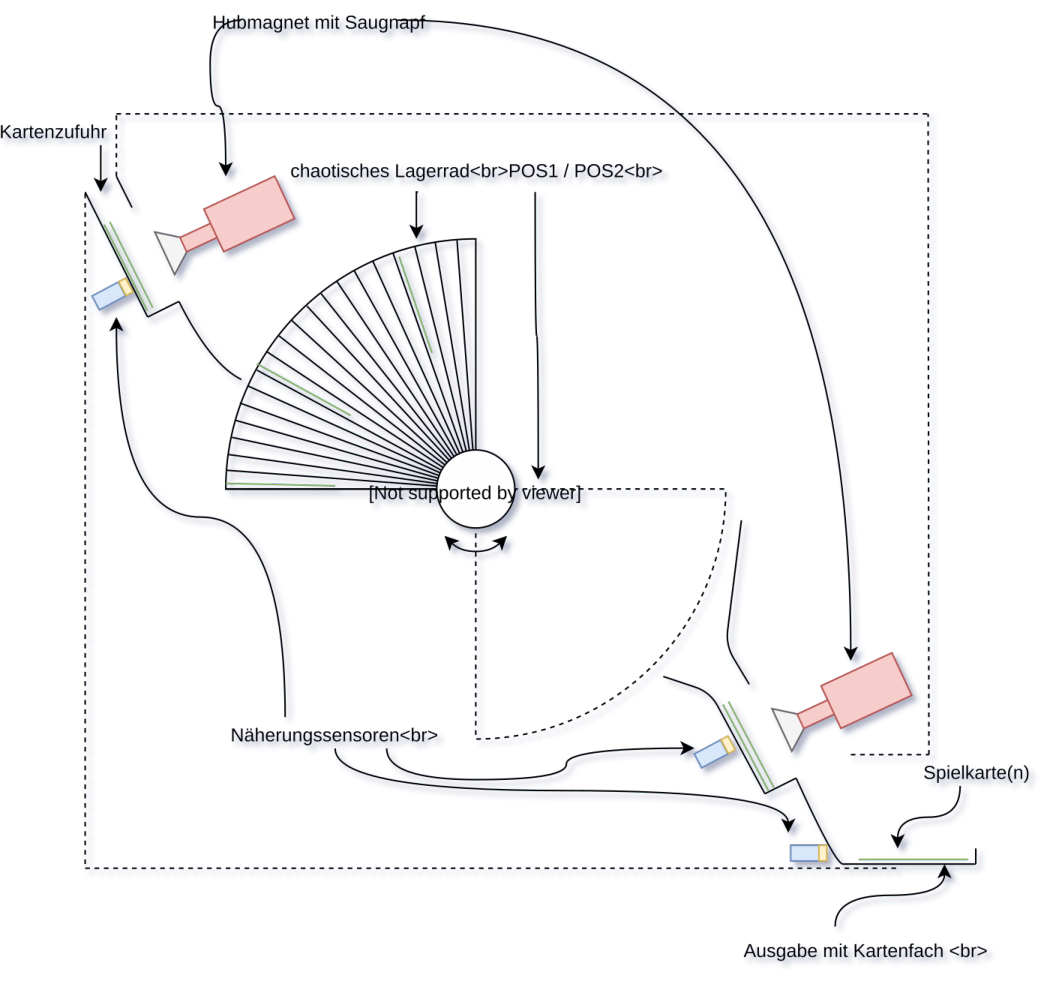
\includegraphics[width=0.6\textwidth]{fig/Reshuffled_Version_3_0_prinzip.pdf}
  \caption{Name des Bildes}
  \label{fig:verweis}
\end{figure}

Grundsätzlich basiert das Mischprinzip auf einer Art "Fächersystem".
Eingelegte Karten gelangen mithilfe eines ausgeklügelten Systems, welches aus einem Hubmagneten mit integriertem Saugnapf besteht, aus dem Einlegefach.
Erfolgt die Kartenentnahme, rutscht die Karte in ein zufälliges Fach des Lagerrads. Anschließend wird dieses Lagerrad in Drehbewegung versetzt um die gelagerten Karten auszugeben.

Der Benutzer steuert diese Maschiene mithilfe einer GUI welche auf einem 7" LCD Display angezeigt wird. Systemintern steuert ein 8-Bit Mikrocontroller der AVR-Familie den Ablauf.

\clearpage

\newpage
\thispagestyle{empty}
\mbox{}

\clearpage

\subsection*{Gender Erklärung}
\label{sec:gender-erklaerung}
Aus Gründen der besseren Lesbarkeit wird in dieser Arbeit die Sprachform des generischen Maskulinums angewendet. Es wird an dieser Stelle darauf hingewiesen, dass die ausschließliche Verwendung der männlichen Form geschlechtsunabhängig verstanden werden soll.

\subsection*{Über dieses Dokument}
\label{sec:ueber-dokument}
Diese Arbeit wurde in \LaTeX{} verfasst. Diese Art der Dokumentation bietet gegenüber den normalen Textverarbeitungen gewisse Vorteile hinsichtlich der Formatierung und des Einbindens von Grafiken. Auch Formeln können sehr einfach und effizient angegegeben werden. Die Rohfassung des Dokuments befindet sich auf dem Arnfelser Gitweb Server der HTBLA Kaindorf Abteilung Mechatronik.

\clearpage

\newpage
\thispagestyle{empty}
\mbox{}

\clearpage

\section*{Projektteam}
\label{sec:projektteam}

\subsection*{Stefan Hörmann}
\begin{wrapfigure}[10]{l}{0.5\textwidth}
\begin{center}
  \includegraphics[width=0.35\textwidth]{fig/logoMecha}
\end{center}
\end{wrapfigure}
\mbox{}\\
\mbox{}\\
\textbf{Aufgabenbereich}:\\
Mechanik\\
\textbf{Betreuer}:\\
Dr. Dipl-Ing. Gerhard Pretterhofer
\mbox{}\\
\mbox{}\\
\mbox{}\\
\mbox{}\\
\mbox{}\\
\mbox{}\\

\subsection*{Nicolas Perl}
\begin{wrapfigure}[10]{l}{0.5\textwidth}
\begin{center}
  \includegraphics[width=0.35\textwidth]{fig/logoMecha}
\end{center}
\end{wrapfigure}
\mbox{}\\
\mbox{}\\
\textbf{Aufgabenbereich}:\\
Elektronik\\
\textbf{Betreuer}:\\
Dipl-Ing. Manfred Steiner
\mbox{}\\
\mbox{}\\
\mbox{}\\
\mbox{}\\
\mbox{}\\

\subsection*{Alois Vollmaier}
\begin{wrapfigure}[10]{l}{0.5\textwidth}
\begin{center}
  \includegraphics[width=0.35\textwidth]{fig/logoMecha}
\end{center}
\end{wrapfigure}
\mbox{}\\
\mbox{}\\
\textbf{Aufgabenbereich}:\\
Informatik\\
\textbf{Betreuer}:\\
Dipl-Ing. Manfred Steiner
\mbox{}\\
\mbox{}\\
\mbox{}\\
\mbox{}\\
\mbox{}\\
\mbox{}\\